\documentclass{article}
\usepackage[T1]{fontenc}
\usepackage{lmodern}
\usepackage{graphicx}
\usepackage{amsmath,amssymb}
\usepackage[a4paper,margin=2cm]{geometry}
\usepackage[absolute,overlay]{textpos}
\setlength{\TPHorizModule}{1mm}
\setlength{\TPVertModule}{1mm}
\usepackage[indonesian]{babel}
\usepackage{hyperref}
\setlength{\emergencystretch}{2em}
% unit: Halaman 18

\begin{document}

% === Halaman 18 (python/native) ===

Sumber gambar: https://textbook.cs161.org/crypto/key-exchange.html 

•

Gambar man-in-the-middle attack berikut memperlihatkan cara Mallory  menyepakati  

kunci yang sama dengan Alice (K1 = gam  mod p) dan menyepakati kunci yang sama 

dengan Bob  (K2 = gbm mod p)

•

Ketika Alice mengirim ga  mod p kepada Bob, 

Mallory mengintersepsi komunikasi dan 

menggantikannya dengan gm  mod p lalu 

mengirimkannya kepada Bob

•

Ketika Bob mengirim gb  mod p kepada Alice, 

Mallory mengintersepsi komunikasi dan 

menggantikannya dengan gm  mod p lalu 

mengirimkannya kepada Alice.

•

Alice menghitung K1 = gam  mod p, sama dengan 

yang dihitung Mallory, K1 = gam  mod p

•

Bob menghitung K2 = gbm  mod p, sama dengan 

yang dihitung Mallory, K2 = gbm  mod p

•

Selanjutnya Mallory mengetahui pesan2 rahasia 

dari Alice dan dari Bob yang diekripsi dengan 

dengan kunci K1 dan K2 tersebut

Rinaldi M/II4020 Kriptografi

18

% deskripsi: gambar native xref 84
\noindent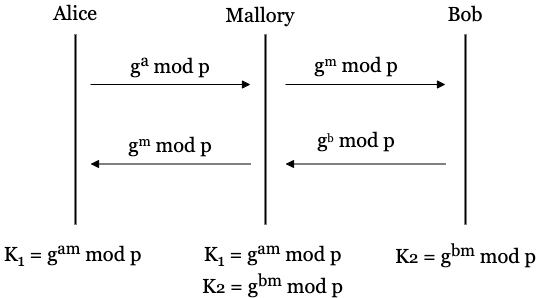
\includegraphics[width=0.85\textwidth]{../../images/python/page_018_img_01.png}

\end{document}
